\section{Control Rights and Preventive Demands}\label{sec:control}

The static model holds Europe's exit premium fixed. Yet the premium moves: Chinese offers and European rearmament raise it, and Chinese indigenization lowers it. A Washington that expects it to turn positive expects to pay rents that Europe cannot credibly promise to forgo. A transfer of control can remove them.

\subsection{Setup}\label{sec:controlsetup}

There are two periods, $t\in\{1,2\}$, and a discount factor $\delta\in(0,1]$. In each period in which Europe holds control, the bidding contest of \cref{lem:bidding} is played at that period's premium $Q_t$, and Europe receives $\pos{Q_t}$. We assume that Washington retains Europe at every contest, including after a cut ($Q_1+d_1<V$ and $Q_1+d_1\le\bar m_U$, and the same in period 2 at the highest premium Europe can reach), and that payments are made at signing.

\paragraph{The ultimatum.} At the start of period 1, before the period-1 contest, Washington may issue an ultimatum at an issuing cost $\iota\ge 0$: Europe transfers control of ASML's customers, output and technology for both periods against a payment $T\ge 0$, or Washington withdraws a bundle $J$ of instruments for period 1. The bundle has unconditional part $u_1$, conditional part $d_1$ and direct ex post cost $g_1\ge 0$ to Washington (\cref{sec:commitment}). If Europe refuses and the threat is carried out, Europe's premium rises to $Q_1+d_1$, and by \cref{prop:slack}(a) the refusal costs Europe the bite
\[
B_1=u_1+\min\{d_1,\Lambda_1\},\qquad \Lambda_1=\pos{-Q_1},
\]
net of the rent Washington must then pay. Carrying out the threat costs Washington $e=g_1+\pos{Q_1+d_1}-\pos{Q_1}$, its direct cost plus the extra rent. The threat is credible if and only if $e\le\bar m_U$; otherwise $B_1=0$. We assume that no other period-1 demand draws on the bite; with other demands, control enters \cref{cor:rationing} as a sunk demand.

We do not expect the core guarantee to back such an ultimatum. Withdrawing protection from a Europe that stays aligned costs Washington its own stake in defending a loyal ally, so $g_1$ is large unless $s_A$ is small. Posture, enablers and the AI instrument cost less to withdraw for one period.

\paragraph{Control.} A transfer lowers Europe's premium at both dates by $\Delta_c\in(0,\infty]$, the enforceability of control. With $\Delta_c=\infty$ Europe can never again choose exit. With $\Delta_c$ finite, a Europe whose premium later rises far enough could take back part of what it gave. What is transferred sets $\Delta_c$. Relocating capacity to US soil raises it, and so does control exercised through ASML's US subsidiaries, which are US-law entities \citep{asml2026subsidiaries}. A controlling vote in a Dutch holding company stays under Dutch law and has low $\Delta_c$; we think it would be exposed to emergency powers like the Goods Availability Act order against Nexperia of 30 September 2025 \citep{kst32637720}.

\paragraph{Values and costs.} Washington places an intrinsic value $v_c\ge 0$ on control, apart from the rents it saves. Europe bears a sovereignty cost $\sigma\ge 0$ if it transfers control. It includes the domestic cost of surrendering a national champion and hurdles fixed in advance: ASML's preference-share foundation, screening under the Vifo Act (\cref{sec:background}), and review under the Foreign Subsidies Regulation, which we infer a US-funded acquisition would trigger \citep{eu2022fsr}. Being public, these hurdles raise $\sigma$ before Washington decides whether to demand anything. China punishes a completed transfer with $r^c\ge 0$, which Europe bears.

\paragraph{Autonomy investment.} After the period-1 outcome, and before the period-2 contest, Europe can make an observable investment at cost $K$ that raises its period-2 premium by $\bar I$, for instance rearmament that lowers $S_k$. Holding a period-2 premium $q$, it invests if and only if $\delta(\pos{q+\bar I}-\pos{q})>K$.

\paragraph{Ties.} An indifferent Europe accepts; Washington issues only if it strictly gains (the limit $\iota\to 0^{+}$ when $\iota=0$); Europe invests only if that is strictly profitable. After a transfer Washington keeps its baseline provision, since withdrawing it would cost something and gain nothing.

\subsection{Preventive control}\label{sec:preventive}

Let $I(q)=\mathbf 1\{\delta(\pos{q+\bar I}-\pos{q})>K\}$ indicate investment at period-2 premium $q$. Washington's discounted period-2 rent is $\mathrm{Rent}_U(q)=\delta\pos{q+\bar I\,I(q)}$, and Europe's period-2 value net of its investment cost is $\mathrm{Val}_H(q)=\mathrm{Rent}_U(q)-K\,I(q)$.

\begin{proposition}[Preventive control]\label{prop:control}
Let
\begin{align*}
\Delta R_U&=\pos{Q_1}-\pos{Q_1-\Delta_c}+\mathrm{Rent}_U(Q_2)-\mathrm{Rent}_U(Q_2-\Delta_c),\\
\Delta R_H&=\pos{Q_1}-\pos{Q_1-\Delta_c}+\mathrm{Val}_H(Q_2)-\mathrm{Val}_H(Q_2-\Delta_c).
\end{align*}
Let $B_1=u_1+\min\{d_1,\Lambda_1\}$ if the threat is credible ($e\le\bar m_U$, with $e=g_1+\pos{Q_1+d_1}-\pos{Q_1}$) and $B_1=0$ otherwise. In the subgame-perfect equilibrium, the United States issues the ultimatum, and Europe accepts, if and only if
\begin{equation*}
\Gamma\equiv v_c-\iota+\min\{\Delta R_U,\;(\Delta R_U-\Delta R_H)+B_1-\sigma-r^c\}>0 .
\end{equation*}
The payment is $T^*=\pos{\Delta R_H-B_1+\sigma+r^c}$, the United States gains $\Gamma$, and Europe's payoff is
$\max\{\Delta R_H-B_1,\,-\sigma-r^c\}+\pos{Q_1-\Delta_c}+\mathrm{Val}_H(Q_2-\Delta_c)$.
An ultimatum that is issued is accepted. The credibility condition $e\le\bar m_U$ does not depend on $\Delta_c$.
\end{proposition}

The proof is in \cref{app:proofs}. $\Delta R_U$ is the rent that control saves Washington and $\Delta R_H$ is what Europe gives up by losing it; they differ only by the investment cost a transfer spares Europe. Washington gains the value of control net of the issuing cost, plus the smaller of the rent saved and what it can extract by force. Europe is paid for the rents it surrenders and the deadweight cost $\sigma+r^c$, less the bite. A refused ultimatum never pays Washington, so the threat is never carried out on the path. Its credibility is judged against a Europe that keeps control, which is why $\Delta_c$ does not enter.

In the special case $v_c=\iota=0$, $\Delta_c=\infty$, $\bar I=0$ and $Q_1<0$, the gain is $\Gamma=\min\{\delta\pos{Q_2},\,B_1-\sigma-r^c\}$. Washington demands control if and only if Europe's future premium is positive and the bite exceeds $\sigma+r^c$. Since $B_1\le u_1+\Lambda_1$, a purely conditional bundle clears that bar only if $Q_1<-(\sigma+r^c)$. The demand comes while Europe is weak but expected to grow stronger.

\begin{corollary}[Motive, investment, enforceability, China]\label{cor:control}
\leavevmode
\begin{enumerate}[label=(\alph*)]
\item \emph{Preventive motive.} $\Gamma>0$ if and only if $\Delta R_U>\iota-v_c$ and $B_1+(\Delta R_U-\Delta R_H)>\sigma+r^c+\iota-v_c$. If $v_c\le\iota$, issuance requires $\Delta R_U>0$ and $B_1+(\Delta R_U-\Delta R_H)>\sigma+r^c$. For $\Delta_c>0$, $\Delta R_U>0$ if and only if $Q_1>0$ or $Q_2+\bar I\,I(Q_2)>0$: Europe's premium is positive at date 1, or its premium after its own investment is positive at date 2.
\item \emph{Autonomy investment.} $\Delta R_U-\Delta R_H=K\,[I(Q_2)-I(Q_2-\Delta_c)]\ge 0$. Both arguments of the minimum in $\Gamma$ are weakly larger than when Europe has no investment option ($\bar I=0$), so an autonomy investment that Europe cannot commit to forgo weakly raises $\Gamma$. With investment, the United States can obtain control with no bite at all: if $B_1=0$, the ultimatum is issued if and only if $\Delta R_U>\iota-v_c$ and $K[I(Q_2)-I(Q_2-\Delta_c)]>\sigma+r^c+\iota-v_c$, and the transfer then saves Europe's investment cost.
\item \emph{Enforceability.} Holding $\sigma$, $r^c$, $v_c$ and $\iota$ fixed, $\Gamma$ and $T^*$ are nondecreasing in $\Delta_c$; $B_1$ and the credibility condition do not depend on $\Delta_c$.
\item \emph{Counter-threats against a transfer.} Before the United States decides, China announces a punishment $r^c\in[0,\bar r^c]$ of a transfer and a stake $m_C\le\bar m_C$. Carrying out $r^c$ after a transfer has ex post value $-e^C(r^c)$ to China, where $e^C$ is continuous and increasing with $e^C(0)=0$; the threat is credible if and only if $e^C(r^c)\le m_C$. China gets $z_C\ge 0$ if Europe keeps control, and the ex post payoff of its punishment decision ($-e^C(r^c)$ if it punishes, $-m_C$ if it does not) if control passes. Write $\Gamma(r^c)$ for $\Gamma$ at punishment $r^c$, and let $r^c_{\max}=\max\{x\le\bar r^c:e^C(x)\le\bar m_C\}$. In every subgame-perfect equilibrium:
\begin{enumerate}[label=(\roman*)]
\item if control is transferred, China does not punish: on the path the punishment is zero, the payment is $\pos{\Delta R_H-B_1+\sigma}$ and $\Gamma(0)>0$;
\item a credible punishment $r^c>0$ is announced only if it deters, $\Gamma(r^c)\le 0$;
\item if $z_C>0$, control is transferred if and only if $\Gamma(r^c_{\max})>0$; otherwise China deters with a credible $r^c\ge v_c-\iota+\Delta R_U-\Delta R_H+B_1-\sigma$ whenever $\Gamma(0)>0$;
\item if $z_C=0$ and $\Gamma(0)>0\ge\Gamma(r^c_{\max})$, both the transfer and its deterrence are equilibrium outcomes.
\end{enumerate}
If punishing is self-rewarding ($e^C(x)<0$ for some $x$), (i) fails: China may let the transfer happen and punish it.
\end{enumerate}
\end{corollary}

When $v_c=0$ and Europe has no autonomy investment that a transfer would forestall, an accepted transfer is inefficient. The rents it avoids are transfers between Washington and Europe, while the sovereignty cost and the issuing cost are destroyed, and China's punishment adds to the loss when, being self-rewarding, it is carried out (part (d)). That is the logic of preventive war \citep{fearon1995rationalist, powell2006war}, with a coerced transfer in place of a war. With an investment option the transfer can be efficient, because it spares Europe an investment cost $K$ sunk only to secure rents (part (b)), the one place where the logic of \citet{grossman1986costs} operates in our model. What our setting adds to the models of \cref{sec:literature} is a ceiling on coercion: the conditional part of the bite cannot exceed Europe's current slack, so the patron must act while the holder is weak.

Part (b) ties the demand to Europe's own choices. An investment in future bargaining power that Europe cannot commit to forgo invites the demand, as an observable nuclear programme invites prevention or a deal \citep{debs2014known, spaniel2019bargaining}. It raises the rents a transfer saves and creates a surplus the two can share, which permits a purchase with no bite. Take $\delta=1$, $Q_1=1$, $Q_2=-\tfrac12$, $\bar I=3$, $K=2$, $\Delta_c=\infty$, $\sigma=1$ and $r^c=v_c=\iota=0$, with no threat. Europe would invest, so Washington faces a period-2 rent of $2.5$ on top of the period-1 rent of $1$. It buys control for $T^*=2.5$ and gains $\Gamma=1$; the transfer spares an investment of $2$ at a sovereignty cost of $1$. Rearmament that Europe cannot commit to forgo can therefore prompt an offer for the chokepoint itself.

By part (c), a transfer that Europe could partly undo removes only $\min\{\pos{Q_t},\Delta_c\}$ of the rent at each date, so the commitment problem returns whenever $Q_2-\Delta_c>0$, and Washington gains less and pays less, the buy-or-lease logic of \citet{harstad2016market}. Relocating production is the high-$\Delta_c$ end. The control rights Washington has taken so far all attach to assets on US soil, where enforcement does not depend on a foreign government: consent rights over the ownership, exit and customers of MP Materials, bought with equity, a price floor and an offtake \citep{mp2025dod}, a golden share in US Steel as a condition of its acquisition by Nippon Steel \citep{ussteel2025nsa}, and a passive stake in Intel \citep{intel2025agreement}. Toward Taiwan, Washington has sought relocation (\cref{sec:cases}).

By part (d), China's threat to punish a transfer is never carried out on the path: once control has passed, punishing costs China something and deters nothing. The threat protects European ownership only by deterring the demand, which requires $\Gamma(r^c_{\max})\le 0$. Sovereignty costs work the same way, which makes the hurdles of \cref{sec:controlsetup} part of Europe's protection against a demand.

\subsection{Windows}\label{sec:windows}

\Cref{prop:control} allows one ultimatum and a one-period cut. When a cut runs over several dates, its bite is the discounted sum of the per-date bites $u_s+\min\{d_s,\Lambda_s\}$, provided Washington retains Europe throughout (\cref{lem:selflimit} in \cref{app:cuts}). A cut is spent once executed, and extending a purely conditional cut into a date at which Europe's premium is positive adds nothing to its bite. A threat of permanent exclusion therefore bites no harder than one confined to the dates at which Europe has slack.

\begin{corollary}[Windows]\label{cor:windows}
Consider $N$ dates with $v_c=0$ and $\Delta_c=\infty$. At any date $t$ at which Europe still holds control, the United States may issue, at cost $\iota>0$, an ultimatum: transfer control for all remaining dates against a payment $T\ge 0$, or face a cut at date $t$ only, with bite $b_t=u_t+\min\{d_t,\Lambda_t\}$ and execution cost $e_t=g_t+\pos{Q_t+d_t}-\pos{Q_t}$. Call $t$ \emph{eligible} if $e_t\le\bar m_U$, $b_t>\sigma+r^c$, and $Q_{t'}>0$ for some $t'\ge t$. There is $\bar\iota>0$ such that for every $\iota\in(0,\bar\iota)$, the United States issues an ultimatum on the equilibrium path if and only if some date is eligible. Every ultimatum issued is accepted, and the first one comes no later than the last eligible date (possibly at a date that is not eligible). The same holds at $\iota=0$ when the United States issues only if it strictly gains. If $u_t=0$ at every date, the condition $t'\ge t$ can be replaced by $t'>t$.
\end{corollary}

\begin{figure}[t]
\centering
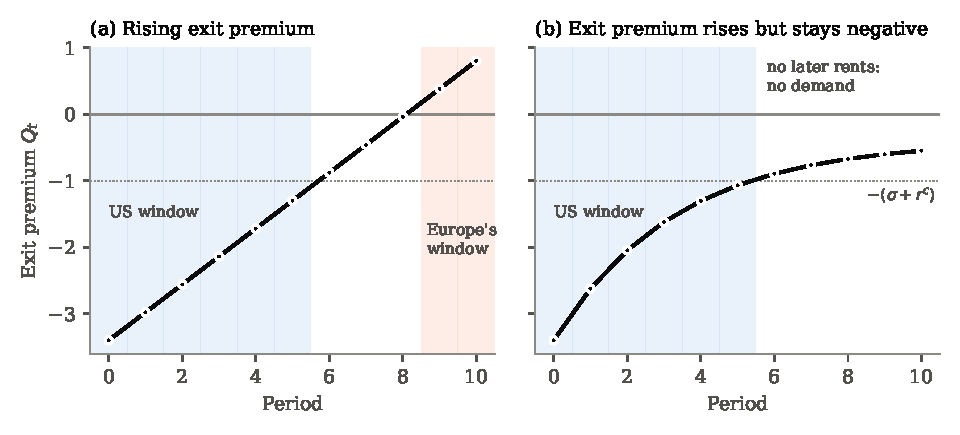
\includegraphics[width=0.95\textwidth]{figures/fig_windows.pdf}
\caption{Windows for preventive control (illustrative units). Panel (a): $Q_t=-3.4+0.42\,t$. Panel (b): $Q_t=-3.4+3(1-e^{-0.3t})$. In both, $\sigma+r^c=1$ and Washington holds a conditional instrument with $d_t=2$ and no unconditional part, so the condition $t'>t$ of \cref{cor:windows} applies; the cut is assumed credible at every date. Blue shading marks dates at which the threat bites by more than $\sigma+r^c$, which here requires $Q_t<-1$. Orange shading marks Europe's window, $Q_t>0$.}
\label{fig:windows}
\end{figure}

In panel (a) of \cref{fig:windows} the threat bites by more than $\sigma+r^c$ through $t=5$, and the premium turns positive at $t=9$. Washington acts at or before $t=5$, long before Europe's window opens. It can act earlier still, because a Europe that refuses remains exposed to a later demand (\cref{app:numerics} reports how often). In panel (b) the premium rises toward $-0.4$ but never crosses zero, and with $v_c=0$ Washington has nothing to prevent; with $v_c>\iota$ it could still demand control (\cref{cor:control}(a)).

In \citet{powell2006war} preventive war requires a shift in power that is large and rapid relative to what the declining state can be offered within the period. Here, under complete information, the speed of the shift affects when Washington acts and what it pays, and not whether it acts, because a transfer with $\Delta_c=\infty$ removes every future rent at once. With finite enforceability a shift far above $\Delta_c$ leaves rents that no transfer can reach, and size and speed matter again, as in Powell's account.

The direction of drift is therefore decisive. Rearmament and the rationing of loyal allies invite a demand, while Chinese indigenization, by lowering $W$, removes the motive. We cannot tell from the record which dominates.

\subsection{Promises or threats}\label{sec:bind}

Europe could instead remove the commitment problem itself, by binding itself against exit without transferring control. Binding also raises Europe's slack and with it the bite of Washington's threats.

\begin{remark}[Self-binding and dual key]\label{rem:bind}
Before period 1, Europe can adopt a binding rule (Europeanized or treaty-entrenched controls) that lowers its premium at both dates by $\Delta_b\in(0,\infty]$ at cost $\sigma^b$, drawing a Chinese punishment $r^b$; Europe keeps the key. The game of \cref{prop:control} is then played with premia $Q_t-\Delta_b$, and the bite of the US threat is computed at the new slack.
\begin{enumerate}[label=(\alph*)]
\item With $\Delta_b=\infty$, control removes no rents, and the bite becomes $B_1^b=u_1+d_1$ if $g_1\le\bar m_U$ (and $0$ otherwise). The United States then issues if and only if $\Gamma^b=v_c-\iota+\min\{0,\,B_1^b-\sigma-r^c\}>0$, so binding pre-empts the ultimatum if and only if $v_c\le\iota$ or $v_c-\iota+B_1^b\le\sigma+r^c$. If it does not, the United States demands control and pays $\pos{\sigma+r^c-B_1^b}$.
\item Let $Q_1<0$, $\Delta_c=\infty$, no investment and $\Delta_b=\infty$. Europe's payoff is $-\sigma^b-r^b-\mathbf 1\{\Gamma^b>0\}\min\{\sigma+r^c,B_1^b\}$ if it binds, and $\max\{\delta\pos{Q_2}-B_1,\,-\sigma-r^c\}$ if it does not bind and $\Gamma>0$, or $\delta\pos{Q_2}$ if it does not bind and $\Gamma\le 0$. In particular, if the United States would issue the ultimatum without binding and binding pre-empts it, Europe strictly prefers to bind if and only if $-\sigma^b-r^b>\max\{\delta\pos{Q_2}-B_1,\,-\sigma-r^c\}$. If the United States would not issue without binding, Europe never strictly prefers to bind.
\item A partial binding ($\Delta_b<\infty$) lowers the rents control would remove but raises the slack, hence the bite, so it can make $\Gamma$ positive. Example, with $\Delta_c=\infty$, no investment and $\bar m_U\ge 1$ (so that the cut is credible after binding): $\delta=1$, $Q_1=-1$, $Q_2=10$, $u_1=0$, $d_1=5$, $g_1=0$, $\sigma=1.5$, $r^c=v_c=\iota=0$. Without binding $\Gamma=\min\{10,\,1-1.5\}<0$. With $\Delta_b=3$, $\Gamma=\min\{7,\,4-1.5\}=2.5$ and the United States demands control at $T^*=4.5$.
\item Dual-key licensing is a partial control transfer with enforceability $\Delta_d<\infty$, sovereignty cost $\sigma_d<\sigma$, value $v_d$ and Chinese punishment $r^d$. If the United States can demand either arrangement, it demands the one with the larger of $\Gamma_{\mathrm{full}}$ and $\Gamma_{\mathrm{dual}}$ (each given by \cref{prop:control} with that arrangement's parameters), provided it is positive. Because $\sigma_d<\sigma$, the United States can obtain a dual key when the bite is too small to obtain full control.
\end{enumerate}
\end{remark}

Binding pre-empts a demand only if Washington values control little for its own sake, since full binding maximizes the bite and makes control cheaper to coerce for a patron with $v_c>\iota$. By part (b), binding pays Europe only when it pre-empts a demand that would otherwise come, at a lower cost. By part (c), a rule that binds Europe partway removes some of the rents Washington fears but adds to the slack its threats draw on, and can turn a demand that would not pay into one that does.

Washington can also demand binding itself. \Cref{prop:control} prices that demand with $(\Delta_b,\sigma^b,r^b)$ in place of $(\Delta_c,\sigma,r^c)$ and $v_c=0$, so a patron that values control little for its own sake prefers to demand binding whenever $\sigma^b+r^b<\sigma+r^c$. A preventive demand need not be a demand for ownership. Under binding Europe holds the only key. Under a dual key Washington holds a veto over China-bound licences, a control right over customers that \cref{rem:bind}(d) prices with its own enforceability and sovereignty cost. The Dutch government's opposition to the extraterritorial reach of the MATCH Act (\cref{sec:background}) suggests to us that $\sigma_d$ in The Hague is not far below $\sigma$, while parliament's 110-to-40 vote in October 2026 for harmonized EU export control \citep{kst37020xvii11} suggests that $\sigma^b$ is low (\cref{sec:record}).

We read the European steps of 2024 and 2025 (\cref{sec:background}) as partial binding. When licensing of the NXT:1970i and NXT:1980i moved from Washington to The Hague in September 2024 \citep{stcrt2024duv}, Europe's premium fell and the key stayed in Europe, the reverse of a control transfer; \cref{sec:coding} codes the December 2024 Supplement No.~4 status as the matching reward for self-binding. On our reading, Delegated Regulation 2025/2003 \citep{eu2025dualuse} raised $\Delta_b$, because removing its entry takes an act at Union level that the Netherlands cannot adopt alone. It also had a US-facing cost. Listed tools ship to US fabs under the Union authorisation EU001 (\cref{sec:background}), so the Netherlands gave up a national licence over their US-bound shipments and, we think, part of Europe's hold-up option (\cref{sec:holdup}). None of these steps comes close to $\Delta_b=\infty$, and by part (c) they could have strengthened the US motive for a demand as easily as weakened it.

\subsection{Private sovereignty costs and breakdown}\label{sec:breakdown}

Under complete information an ultimatum is accepted or never issued. Breakdown requires that Washington be unsure what a transfer would cost Europe. We think that uncertainty is real: since February 2026 the Dutch cabinet has governed with minority support in parliament \citep{nltimes2026coalition, omroepbrabant2026kabinet}, so the domestic price of a transfer would depend on whichever majority it could find. When $\sigma$ is Europe's private information, a threat-backed ultimatum is refused with positive probability and the threat is carried out (\cref{prop:breakdown} in \cref{app:cuts}). Refusal is likelier when China's punishment of a transfer is credible and large, when Europe's future premium is high, and when the threat is cheap for Washington to carry out, the risk-return trade-off of \citet{fearon1995rationalist}. A patron that values control for its own sake may switch from a purchase offer to a threat as the bite rises, which can raise the probability of breakdown. These probabilities describe a patron that can commit to one public demand.
